\documentclass{article}
    % General document formatting
    \usepackage[margin=0.7in]{geometry}
    \usepackage[parfill]{parskip}
    \usepackage[utf8]{inputenc}
    \usepackage{amsmath}
    \usepackage{amssymb}
    \usepackage{tikz}
    \usetikzlibrary{positioning}
    \usepackage{fancyhdr}
    \usepackage{listings}
    \usepackage{multicol}

\pagestyle{fancy}
\fancyhf{}
\rhead{Edgar Jacob Rivera Rios - A01184125}

\begin{document}
\begin{titlepage}

    \newcommand{\HRule}{\rule{\linewidth}{0.5mm}} % Defines a new command for the horizontal lines, change thickness here

    \center % Center everything on the page

    %----------------------------------------------------------------------------------------
    %	HEADING SECTIONS
    %----------------------------------------------------------------------------------------

    \textsc{\LARGE Tecnológico de Monterrey}\\[1.5cm] % Name of your university/college
    \textsc{\Large Computational intelligence}\\[0.5cm] % Major heading such as course name
    %\textsc{\large Minor Heading}\\[0.5cm] % Minor heading such as course title

    %----------------------------------------------------------------------------------------
    %	TITLE SECTION
    %----------------------------------------------------------------------------------------

    \HRule \\[0.4cm]
    { \huge \bfseries Homework 8}\\[0.4cm] % Title of your document
    \HRule \\[1.5cm]

    %----------------------------------------------------------------------------------------
    %	AUTHOR SECTION
    %----------------------------------------------------------------------------------------

    \begin{minipage}{0.4\textwidth}
    \begin{flushleft} \large
    \emph{Student:}\\
    Jacob \textsc{Rivera} % Your name
    \end{flushleft}
    \end{minipage}
    ~
    \begin{minipage}{0.4\textwidth}
    \begin{flushright} \large
    \emph{Professor:} \\
    Dr. José Carlos \textsc{Bayliss} % Supervisor's Name
    \end{flushright}
    \end{minipage}\\[2cm]

    % If you don't want a supervisor, uncomment the two lines below and remove the section above
    %\Large \emph{Author:}\\
    %John \textsc{Smith}\\[3cm] % Your name

    %----------------------------------------------------------------------------------------
    %	DATE SECTION
    %----------------------------------------------------------------------------------------

    {\large \today}\\[2cm] % Date, change the \today to a set date if you want to be precise

    %----------------------------------------------------------------------------------------
    %	LOGO SECTION
    %----------------------------------------------------------------------------------------

    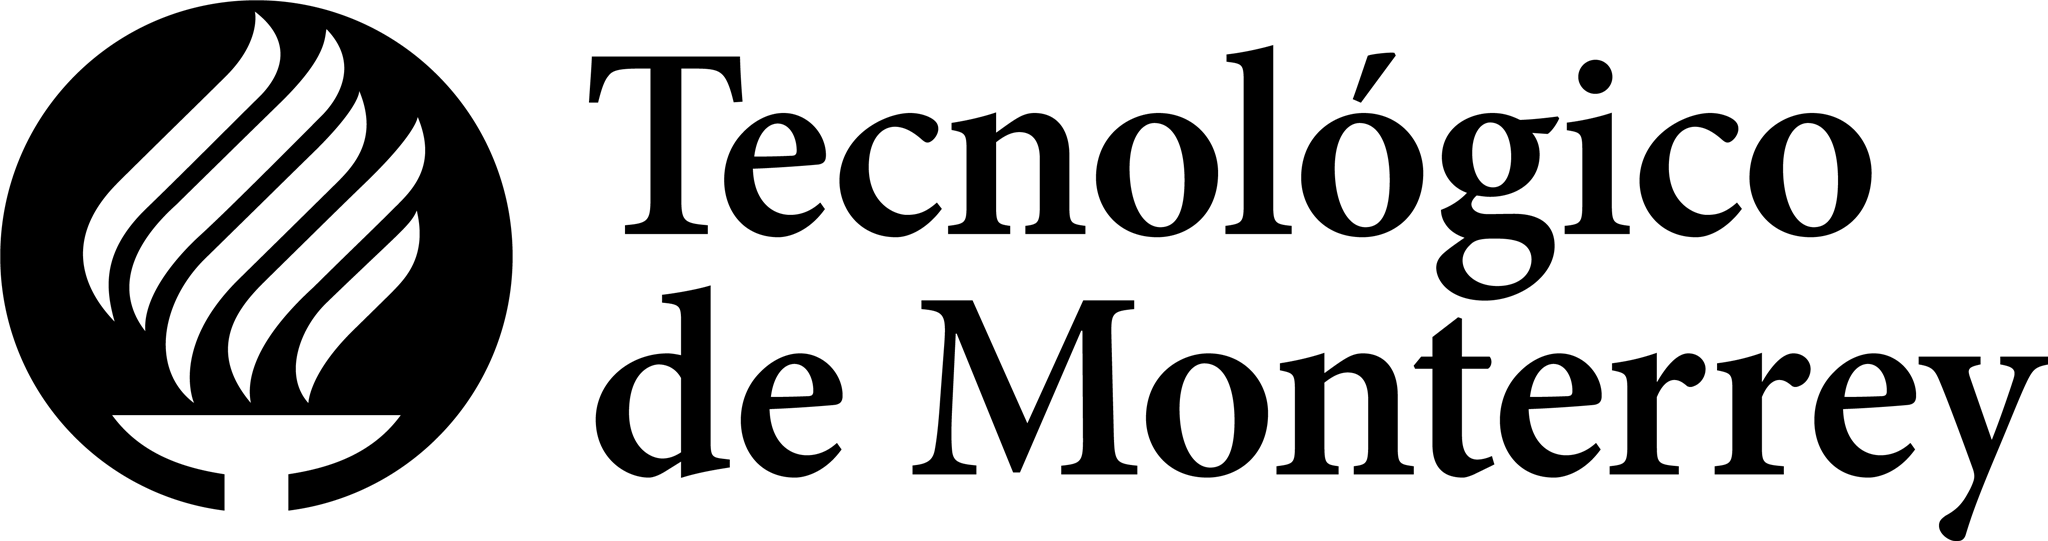
\includegraphics[width=0.4\textwidth,height=\textheight,keepaspectratio]{../Assets/logo-tec-negro.png} % Include a department/university logo - this will require the graphicx package

    %----------------------------------------------------------------------------------------

    \vfill % Fill the rest of the page with whitespace

\end{titlepage}
In this programming assignment you will practice with Kohonen and LVQ neural networks for clustering and classification. For this assignment you are free to use any programming language you choose.
\section{Kohonen network - Analysis}
Suppose that we have a Kohonen network with weight matrix W and we create a new set of weights $W' = cW$ by scaling $W$ by some positive constant $c$. If the Kohonen network now uses $W'$, how would this change affect the network’s decisions? Justify your answer and include an example that supports it.

As this kind of networks try to approach the "centroid" of the input data, an scalation will inevitably move the positions in an undesired way. The form of the weights will stay the same, however, it will be off the real centroid of the input data by a margin tied to $c$. Unless you also scale the inputs by the same constant, knowledge will be lost, altough, easily recuperable.

\section{Learning vector quantization - Analysis}
Given a LVQ network with two inputs and two outputs, provide an example where the simple LVQ training rule will fail to learn how to classify the input (its accuracy will always be zero after the network is trained). Please specify the input data (including the labels), the weights of the network, the labels for the output neurons and a graphical representation of your example. Explain the reasons that make LVQ useless for this particular case (the reasons why it fails to learn) and what changes to the basic LVQ learning method could be implemented in order to properly classify the input.



\section{Kohonen networks and the XOR problem}
We have previously stated in this course that it is not possible for a single-layered perceptron to solve the XOR problem since it is not linearly separable. Now that you know about self-organizing neural networks, do you think is possible for a LVQ neural network to solve the XOR problem? Justify your answer and include an example that supports it.

It is not possible to use it to solve the XOR problem given that the model evaluates the distance between the members and in this case, there exists some equidistance between all the members, even tough they are in separate positions, which can in turn confuse the neural network and not reaching convergence.

\pagebreak
\section{Clustering}
In this assignment you will use a Kohonen neural network to cluster the data contained in the file datasetP4.csv (distributed along with this document).

\begin{itemize}
    \item Plot the data and, by inspection, propose a set of centroids that properly cluster the data.
    \begin{figure}[ht]
        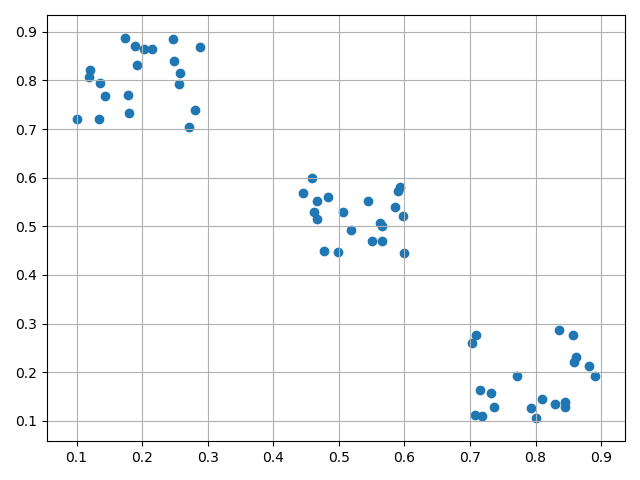
\includegraphics[]{graph.png}        
    \end{figure}
    \begin{itemize}
        \item $(0.2, 0.8)$
        \item $(0.5, 0.5)$
        \item $(0.8, 0.2)$
    \end{itemize}
    \item Write the code to train a Kohonen network and train it for the dataset by using 3, 4, and 5 output neurons. Because the weights are randomly initialized, you will likely run your training process more than once. Among the different runs of the training process, what is the best configuration you obtained? How is the performance of the network affected by the number of output neurons?
    \begin{enumerate}
        \item 3
        \begin{itemize}
            \item $(0.79466, 0.18158)$
            \item $(0.19783, 0.80417)$
            \item $(0.53168, 0.51628)$
        \end{itemize}
        \item 4
        \begin{itemize}
            \item $(0.53168, 0.51628)$
            \item $(0.79466, 0.18158)$
            \item $(0.23460, 0.82816)$
            \item $(0.13824, 0.77079)$
        \end{itemize}
        \item 5
        \begin{itemize}
            \item $(0.20332, 0.86839)$
            \item $(0.26553, 0.80299)$
            \item $(0.53168, 0.51627)$
            \item $(0.13824, 0.77079)$
            \item $(0.79466, 0.18158)$
        \end{itemize}
    \end{enumerate}

    As we can easily see in the graph, there are 3 natural clusters, however, due to the characteristics of the algorithms, we know that the performance artificially increases as the number of clusters grow, as long as it does not surpass the number of items.

    \item Can the Kohonen network properly cluster the dataset? In case your answer is no, justify your answer. In case the Kohonen network successfully clusters all the points in the dataset, provide the values of the weights of such a network as well as the diagram of the network architecture.
    
    Yes, it can do it acurately.
    \begin{figure}[ht]
        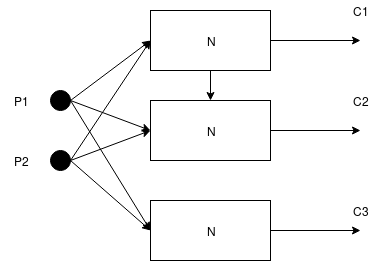
\includegraphics[]{NN.png}        
    \end{figure}
    
    \item How close is the best distribution of the centroids you obtained through the Kohonen network to the distribution you proposed by inspection?
    
    It is very close, as we can easily identify the 3 clusters in the graph. They are fairly concentrated around the proposed centroids and fairly away from each other.

\end{itemize}
\section{Classification}
The following table describes two classes, A and B, which are not linearly separable (for a better inspection of the data, it is highly recommended to plot the classes). This is the same dataset we used in previous homeworks.

\begin{table}
    \centering
    \begin{tabular}{c|c|c}
        x&y&Class\\
        \hline
        -1& 0& 0\\
        0& 1& 0\\
        1& 0& 0\\
        0& -1& 0\\
        -0.5& -0.5& 1\\
        0.5& 0.5& 1\\
    \end{tabular}
\end{table}
\begin{itemize}
    \item  Write the code to train a LVQ neural network. Remember that it is basically a Kohonen network but the learning rule changes so it only updates the weight of the winning neuron if it corresponds to the expected class.
    
    \item Train the LVQ network on the dataset. Because the weights are randomly initialized, you will likely run your training process more than once. Among the different runs of the training process, what is the highest accuracy level you obtained?
    
    \begin{enumerate}
        \item $(-0.024907,  0.776818)$
        \item $(0.747903, -0.108160)$
        \item $(0.396256,  0.179213)$
    \end{enumerate}

    100\% accuracy

    
    \item Can the LVQ network learn the patterns in the dataset? In case your answer is no, justify your answer. In case the LVQ neural network successfully classifies all the patterns in the dataset, provide the values of the weights of such a network as well as the diagram of the network architecture.
    
    It seems that yes, it can learn it, but it is highly vulnerable to the use of different seeds. After some tries, it gave us the correct result.

    \begin{figure}[ht]
        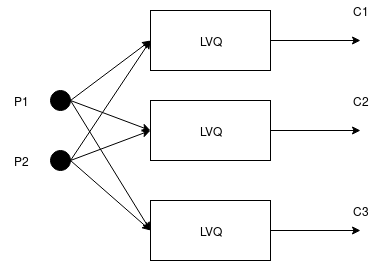
\includegraphics[]{LVQ.png}        
    \end{figure}
    
\end{itemize}

\end{document}